%%%%%%%%%%%%%%%%%%%%%%%%%%%%%%%%%%%%%%%%%%%%%%%%%%%%%%%%%%%%%%%%%%%%%%%%%%%%
%    DO NOT TOUCH (just put your project_proposal.pdf in directory         %
% If the text fields are empty in the pdf, try print to pdf function which %
% can be seen as one of the printing options when trying to print a pdf.   %
% That writes a pdf that removes the fields and only keep the text.        % 
%%%%%%%%%%%%%%%%%%%%%%%%%%%%%%%%%%%%%%%%%%%%%%%%%%%%%%%%%%%%%%%%%%%%%%%%%%%%
\eprsec{Part 2. Project definition: approved Project Proposal}

This section contains the problem identification in the form of the complete approved Project Proposal, unaltered from the final approved version that appears on the AMS.

\addcontentsline{toc}{altsection}{1.\hspace{0.8em}Project description}
\addcontentsline{toc}{altsection}{2.\hspace{0.8em}Technical challenges in this project}
\addcontentsline{toc}{altsection}{3.\hspace{0.8em}Functional analysis}
\addcontentsline{toc}{altsection}{4.\hspace{0.8em}System requirements and specifications}
\addcontentsline{toc}{altsection}{5.\hspace{0.8em}Field conditions}
\addcontentsline{toc}{altsection}{6.\hspace{0.8em}Student tasks}

\mustdo{check these eight pages against the approved proposal on the AMS and confirm that every
answer, the title block and the Feedback block now appear. The included file is a flattened copy;
the original is kept unaltered as \texttt{project\_proposal.pdf}.}

\newpage

% The approved proposal is a PDF form.  \includepdf imports page content but not
% annotations, so the filled-in fields printed as empty boxes.  The included file
% is a flattened copy, produced by tools_flatten_form.py, which draws each
% widget's own /AP /N appearance stream into the page content.  Nothing is
% retyped or altered: the appearances are the ones the form itself carries, so
% Part 2 remains the unaltered approved proposal.  The original form is kept
% beside it as project_proposal.pdf.  Regenerate with:
%   python -I tools_flatten_form.py \
%     2_Project_Definition/project_proposal.pdf \
%     2_Project_Definition/project_proposal_flat.pdf
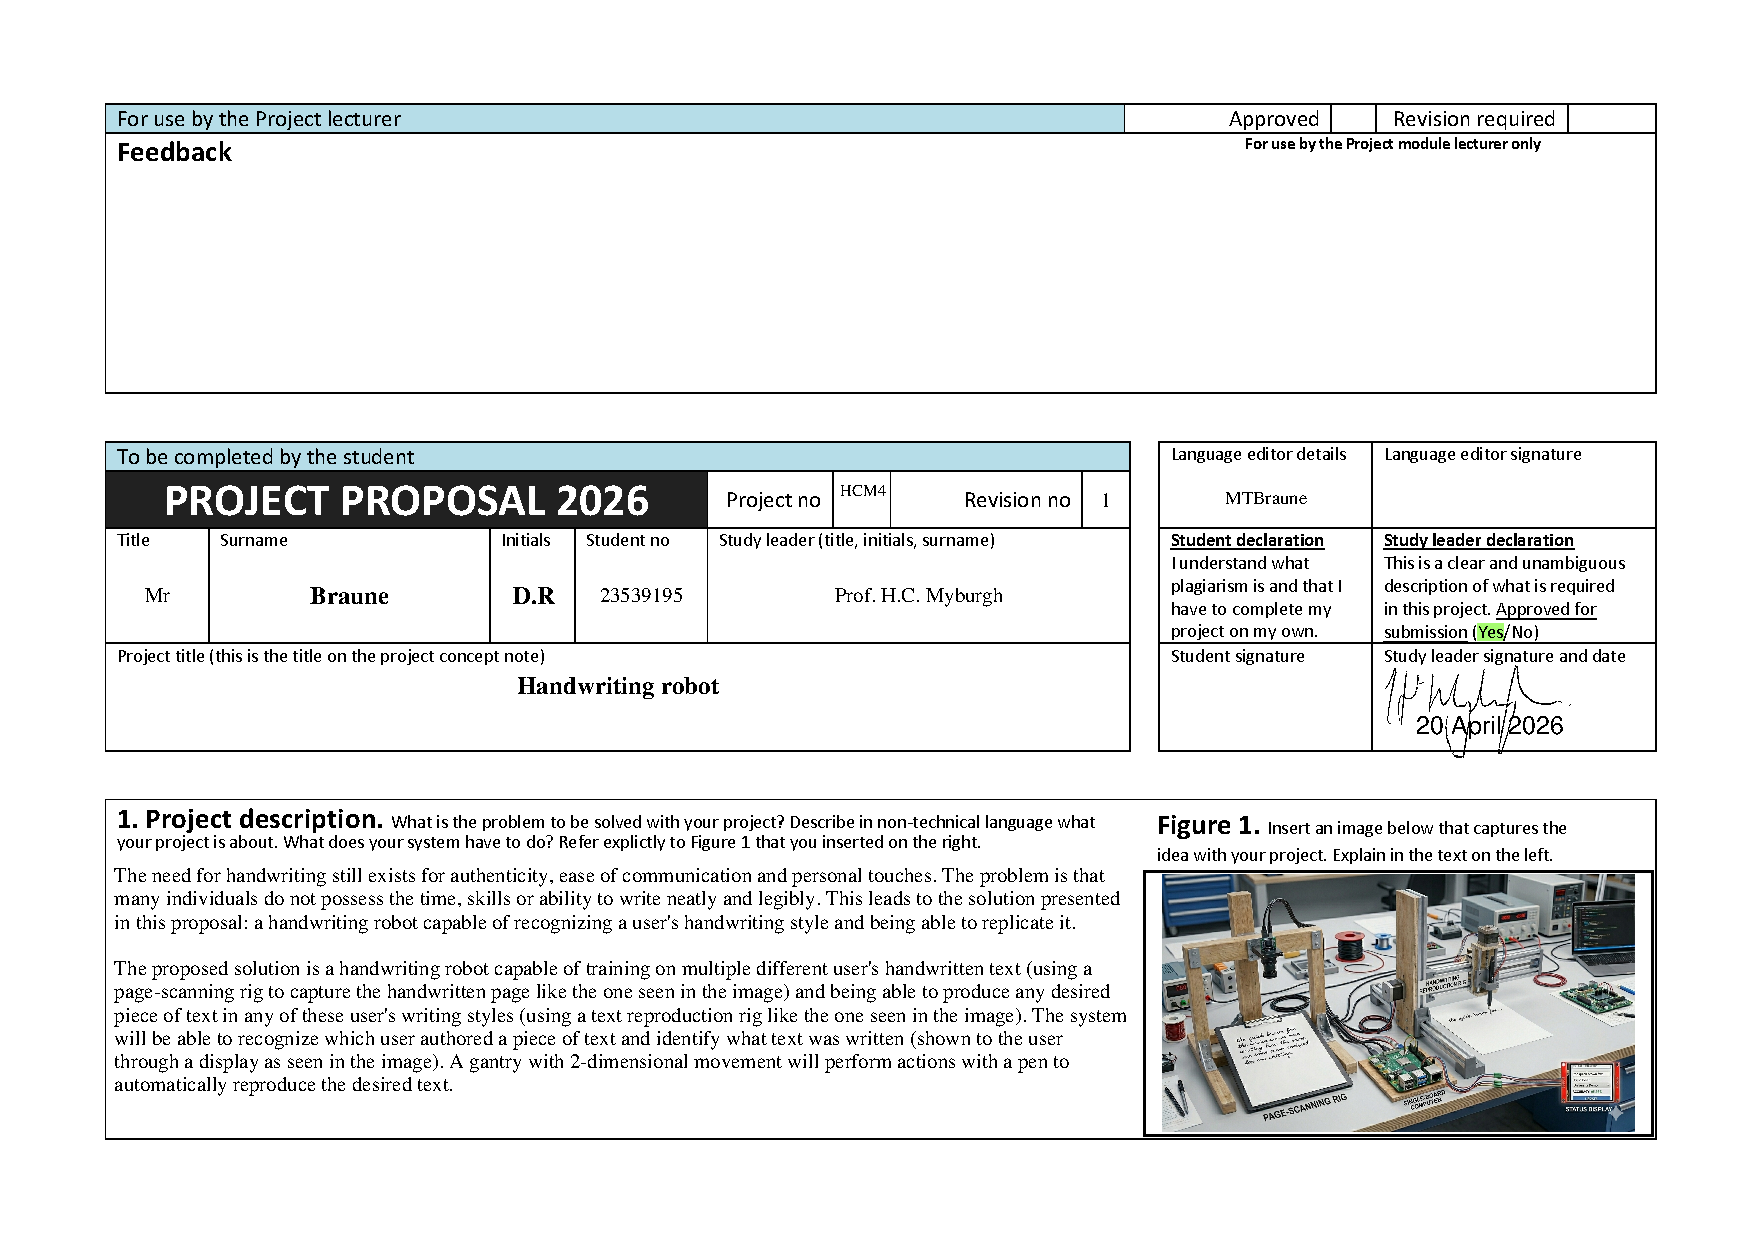
\includepdf[pages=-,landscape]{2_Project_Definition/project_proposal_flat.pdf}
